\section{Scheduling}

\begin{figure}
\centering
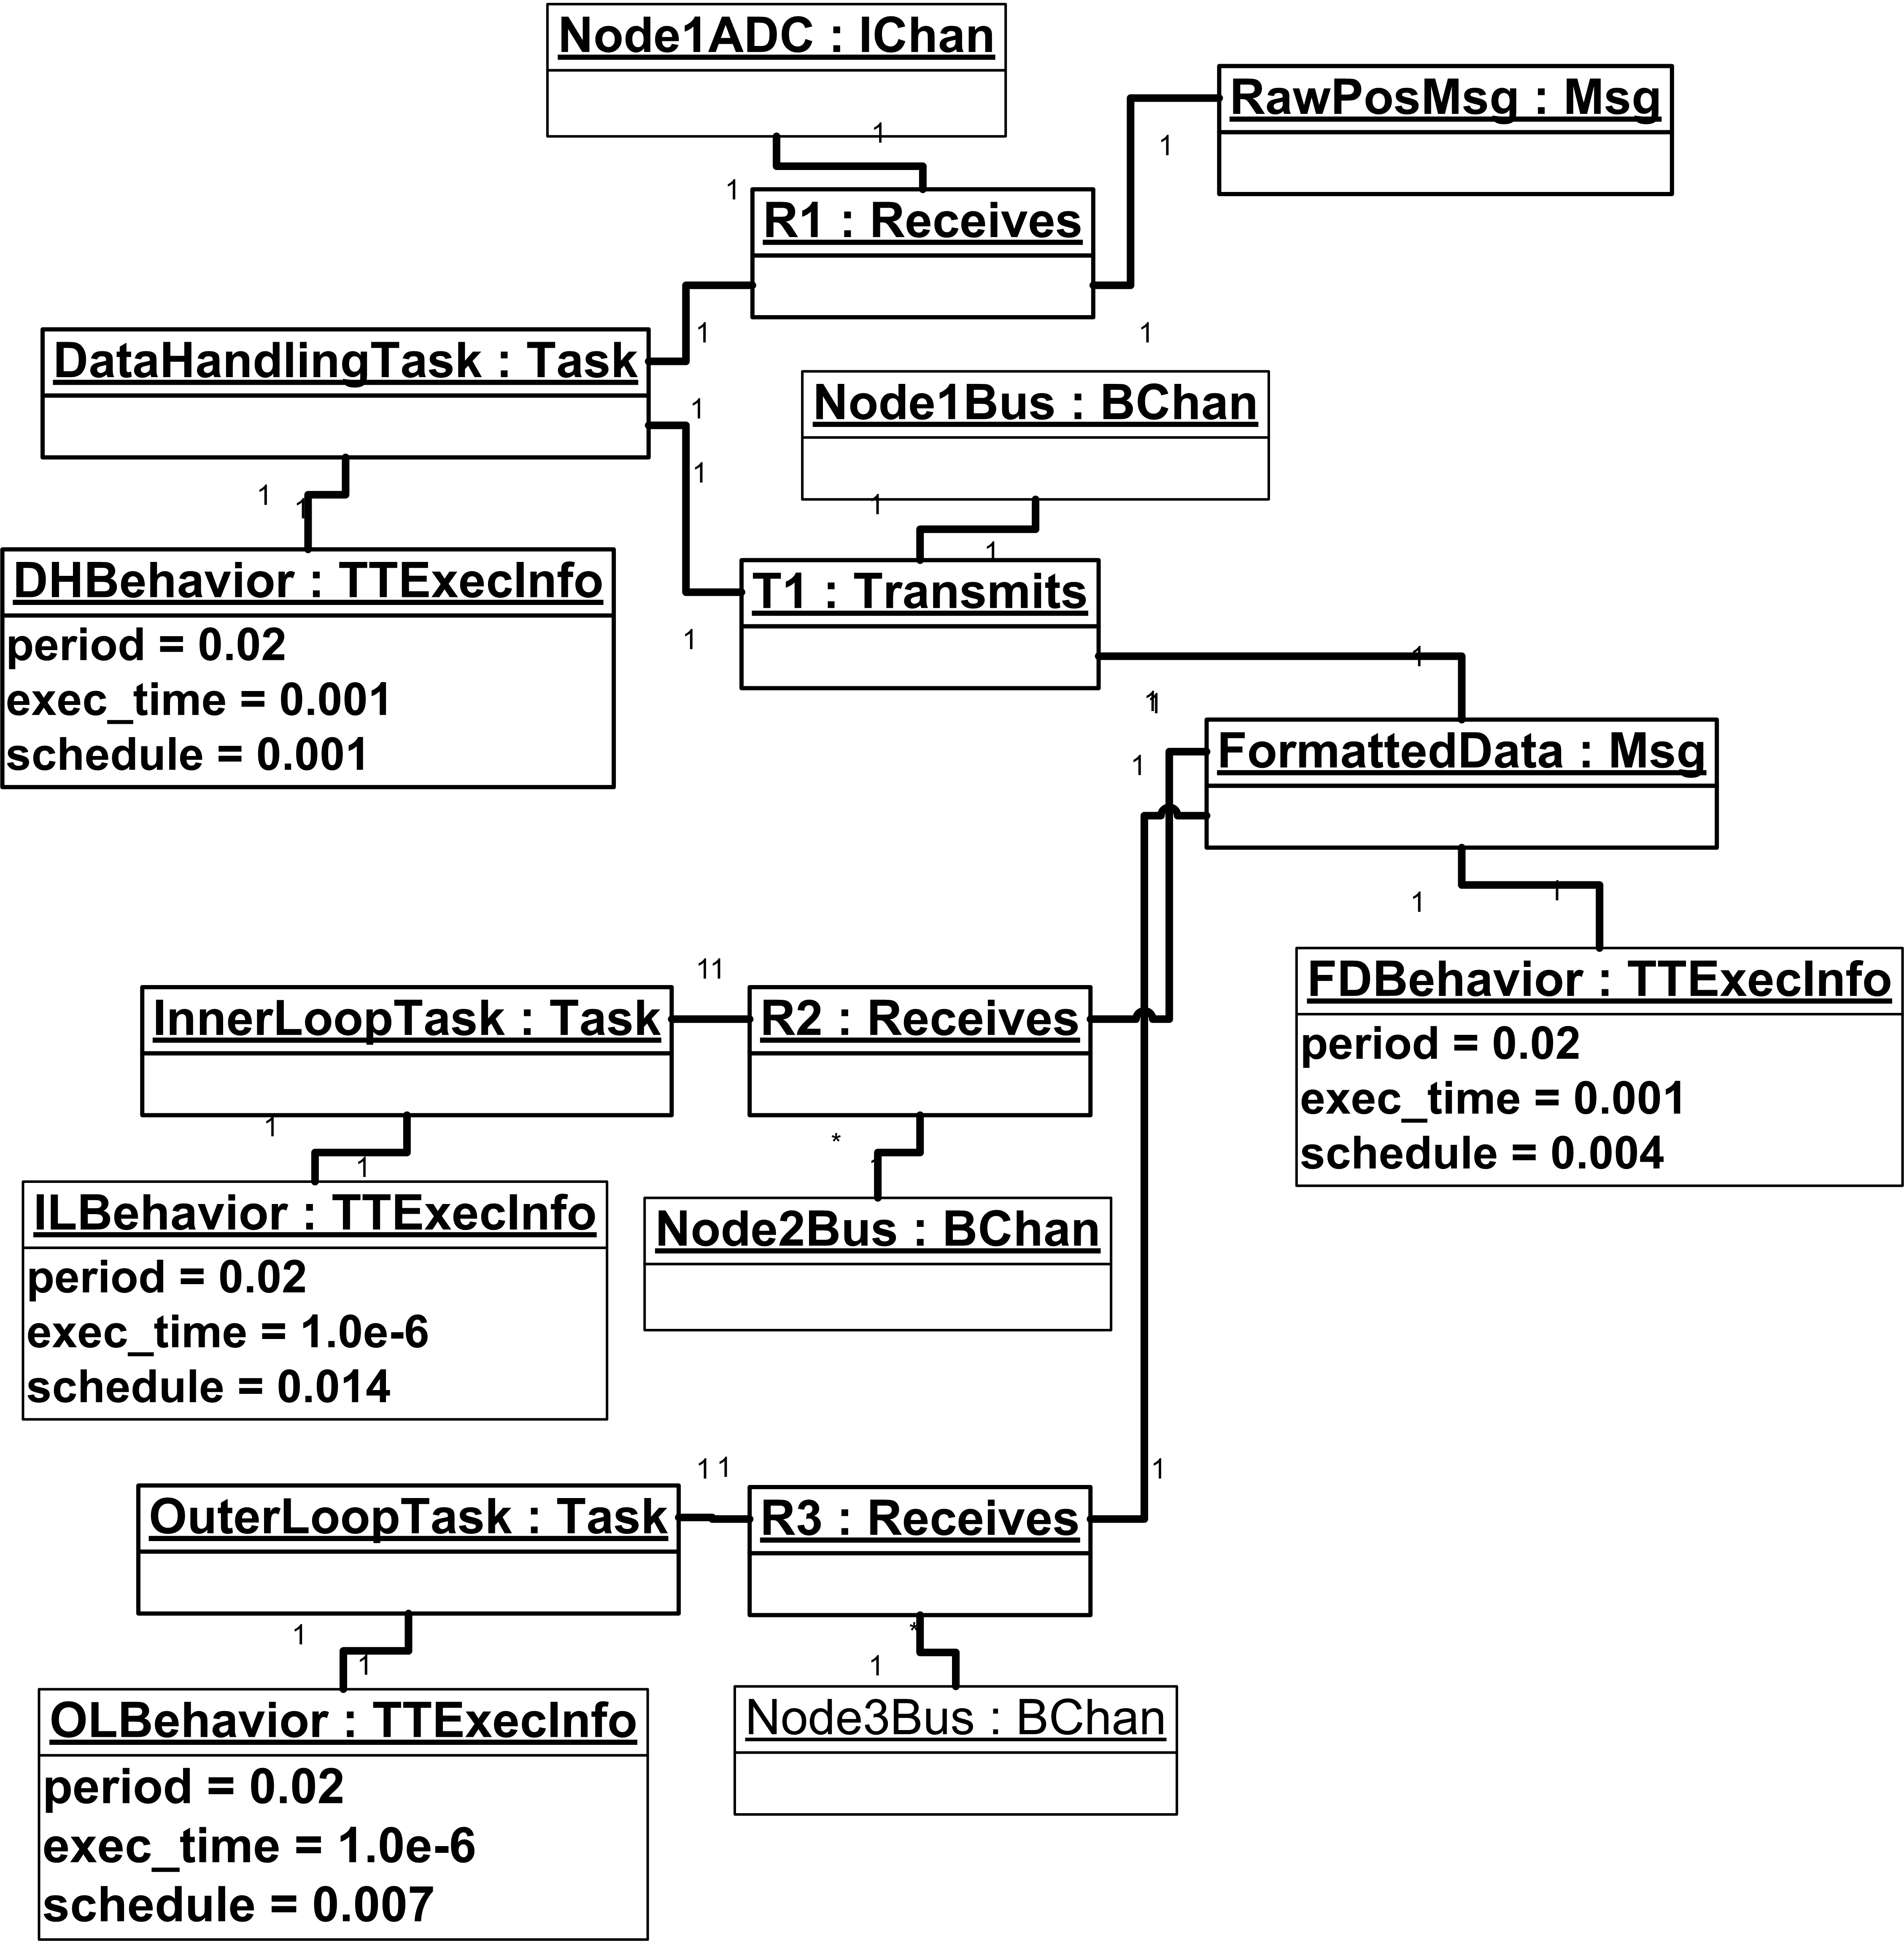
\includegraphics[width=0.87\columnwidth]{figures/msg_struct.png}
    \caption{Semantic model of the message structure from Figs. \ref{fig:deps} and \ref{fig:deploy}. Relation 
objects of type "`Transmits"' and "`Receives"' associate message objects (and their associated behavior objects) 
to sending and receiving tasks, and to node-specific communication channel configurations used to transmit the 
message.  This relation allows us to assemble behavioral information provided by the tasks, messages, and 
platform into a single model.  The schedule interpreter uses information from all of these semantic elements to 
create input for the schedule solver. }
    \label{fig:msg_sched}
\end{figure}


The control design provides task period and execution time specifications for each component instance.  Data 
transfer rates and overhead parameters are found in the platform model.  Messages represent dependencies 
between the tasks.  The semantic model keeps a single set of relations describing the association of task, 
messages, and platform to get a single scheduling model.  Task and message dependencies are given in the 
software architecture model.  \cite{sched:analysis} describes the actual constraint model details.  A constraint 
programming tool solves these constraints for task release times and message transfer times on the time-triggered 
platform. The scheduling process guarantees that the implementation meets the timing requirements required by the 
control design process.  The passive control design provides stability guarantees, even in the face of timing 
jitter or limited message loss.  Hence (within the bounds of acceptable delays) the scheduler does not have to 
account for timing uncertainty beyond that inherent in the platform as long as the component abstraction is 
preserved in all interpretations that use the deployment information.

\begin{figure}
\centering
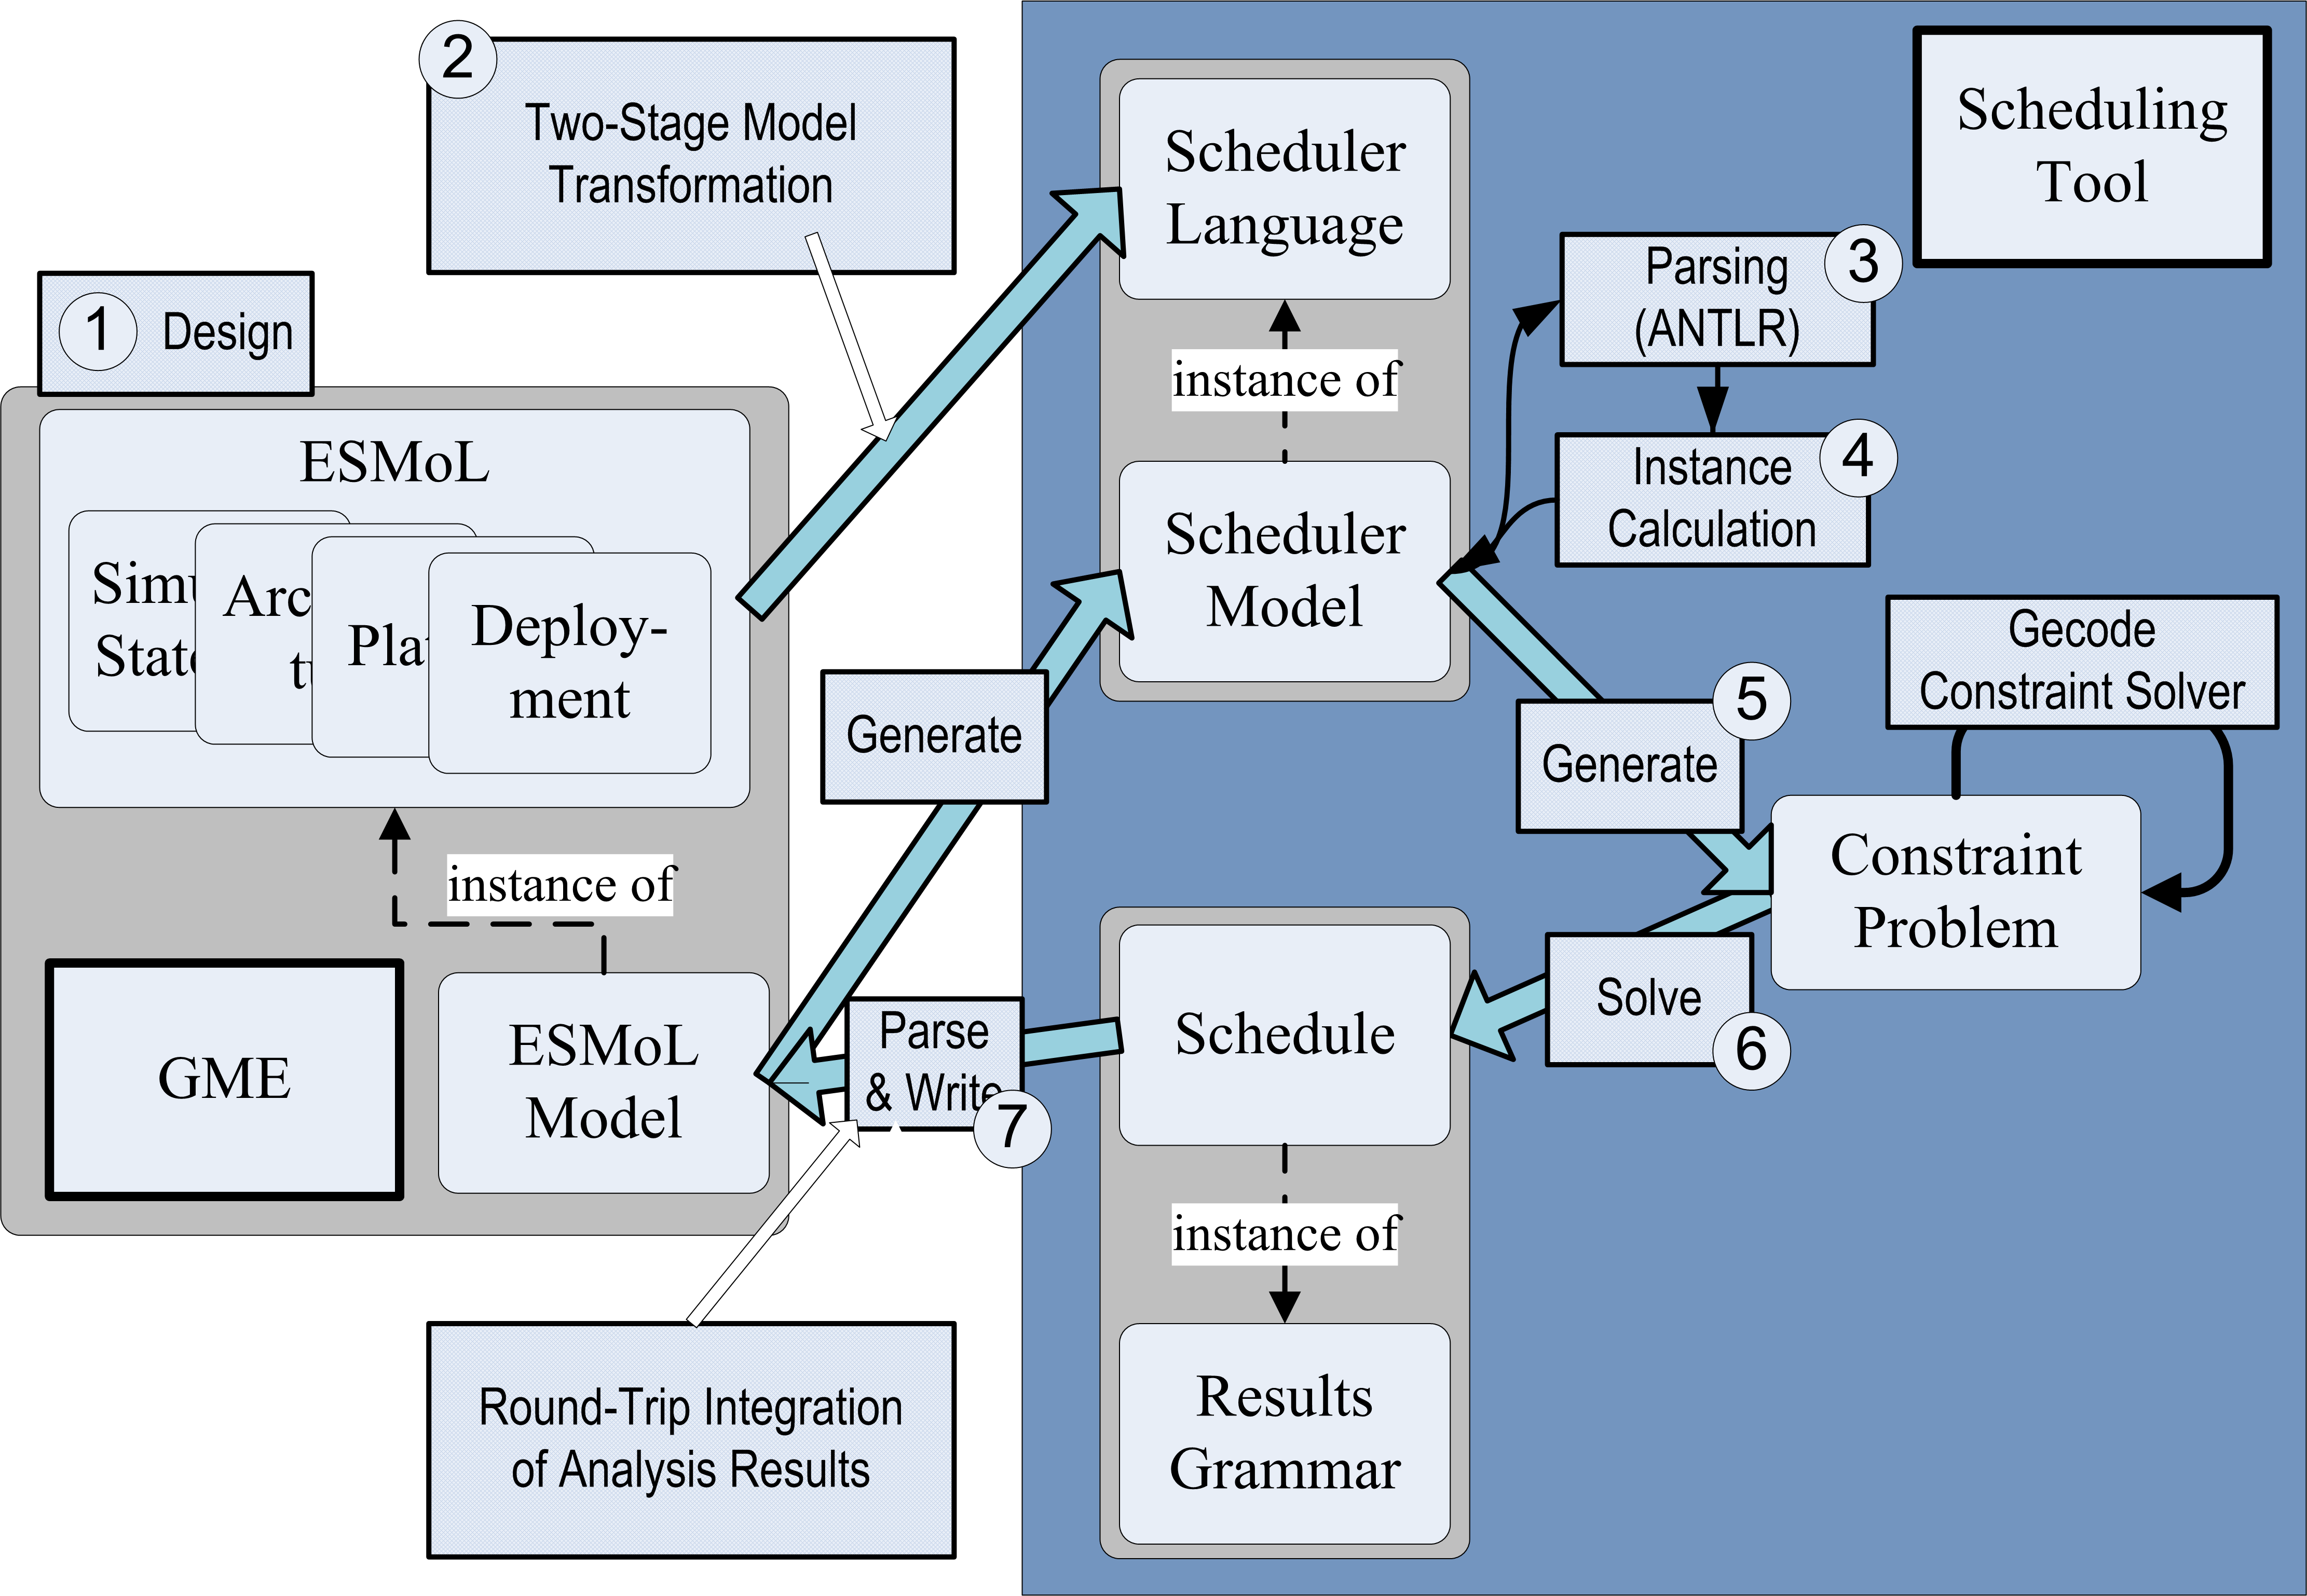
\includegraphics[width=\columnwidth]{figures/sched_integration.png}
    \caption{Integration of the scheduling model by round-trip structural transformation between the language 
of the modeling tools and the analysis language.}
    \label{fig:sched_int}
\end{figure}

As the most mature analysis translator in our tools, the syntactic translation to the scheduling model 
provides the best conceptual illustration of the integration process.  Fig. \ref{fig:sched_int} shows a 
model transformation distilling details from the ESMoL tools and creating a scheduling problem model whose 
syntax represents the proper sets of behaviors.  The task and message release time results (if the schedule 
is feasible) are fed back to the modeling framework as configuration parameters.
